% Star graph
% Author: Anthony Labarre <http://homepages.ulb.ac.be/~alabarre/home.html>
\documentclass{minimal}

\usepackage{tikz}
\usepackage{verbatim}

\begin{comment}

:Title: Star graph
:Author: Anthony Labarre

The star graph of order n has the set of all permutations of {1,2,...,n} as
vertex set and has an edge between any two vertices such that the
corresponding permutations can be obtained from one another by swapping the
first element with any other element (e.g. (1 2 3 4) will be connected to
(3 2 1 4)). This drawing shows the star graph of order 4.

*Note*. You can find many examples of beautiful graphs in Anthony Labarre's publications_ (especially his PhD thesis). Almost all of the graphs have been drawn using TikZ.

.. _publications: http://homepages.ulb.ac.be/~alabarre/publications.html

\end{comment}

\newcommand{\LD}{\langle}
\newcommand{\RD}{\rangle}

\begin{document}

\begin{center}
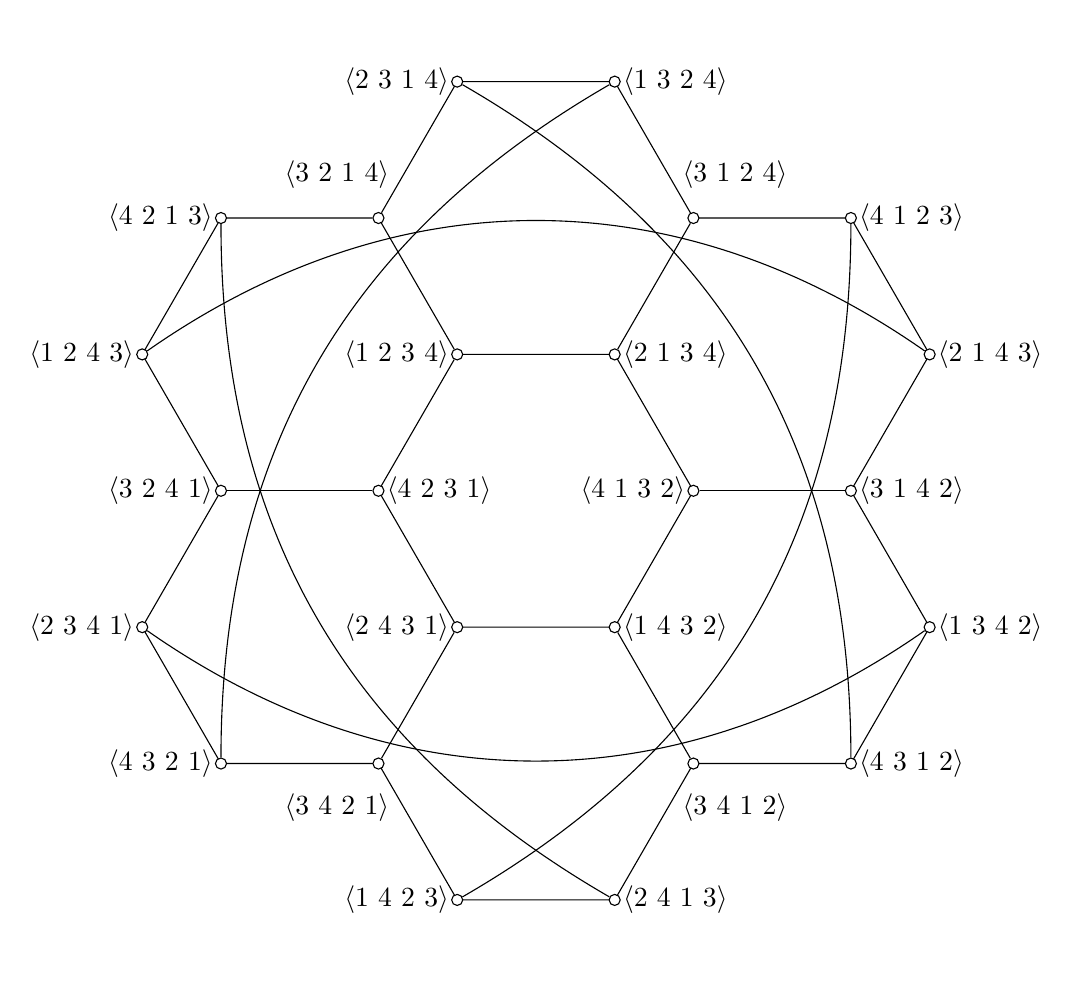
\begin{tikzpicture}
    \tikzstyle{every node}=[draw,circle,fill=white,minimum size=4pt,
                            inner sep=0pt]

    % First, draw the inner hexagon with a ``pin'' -- namely, (3214)
    \draw (0,0) node (1234) [label=left:$\LD 1\ 2\ 3\ 4\RD$] {}
        -- ++(0:2.0cm) node (2134) [label=right:$\LD 2\ 1\ 3\ 4\RD$] {}
        -- ++(300:2.0cm) node (4132) [label=left:$\LD 4\ 1\ 3\ 2\RD$] {}
        -- ++(240:2.0cm) node (1432) [label=right:$\LD 1\ 4\ 3\ 2\RD$] {}
        -- ++(180:2.0cm) node (2431) [label=left:$\LD 2\ 4\ 3\ 1\RD$] {}
        -- ++(120:2.0cm) node (4231) [label=right:$\LD 4\ 2\ 3\ 1\RD$] {}
        -- (1234) % shape is closed, we now connect it to an outer vertex:
        -- ++(120:2.0cm) node (3214) [label=120:$\LD 3\ 2\ 1\ 4\RD$] {};

    % Second, draw the ``outer backbone''
    \draw (3214)
        -- ++(60:2.0cm) node (2314) [label=left:$\LD 2\ 3\ 1\ 4\RD$] {}
        -- ++(0:2.0cm) node (1324) [label=right:$\LD 1\ 3\ 2\ 4\RD$] {}
        -- ++(300:2.0cm) node (3124) [label=60:$\LD 3\ 1\ 2\ 4\RD$] {}
        -- ++(0:2.0cm) node (4123) [label=right:$\LD 4\ 1\ 2\ 3\RD$] {}
        -- ++(300:2.0cm) node (2143) [label=right:$\LD 2\ 1\ 4\ 3\RD$] {}
        -- ++(240:2.0cm) node (3142) [label=right:$\LD 3\ 1\ 4\ 2\RD$] {}
        -- ++(300:2.0cm) node (1342) [label=right:$\LD 1\ 3\ 4\ 2\RD$] {}
        -- ++(240:2.0cm) node (4312) [label=right:$\LD 4\ 3\ 1\ 2\RD$] {}
        -- ++(180:2.0cm) node (3412) [label=-60:$\LD 3\ 4\ 1\ 2\RD$] {}
        -- ++(240:2.0cm) node (2413) [label=right:$\LD 2\ 4\ 1\ 3\RD$] {}
        -- ++(180:2.0cm) node (1423) [label=left:$\LD 1\ 4\ 2\ 3\RD$] {}
        -- ++(120:2.0cm) node (3421) [label=-120:$\LD 3\ 4\ 2\ 1\RD$] {}
        -- ++(180:2.0cm) node (4321) [label=left:$\LD 4\ 3\ 2\ 1\RD$] {}
        -- ++(120:2.0cm) node (2341) [label=left:$\LD 2\ 3\ 4\ 1\RD$] {}
        -- ++(60:2.0cm) node (3241) [label=left:$\LD 3\ 2\ 4\ 1\RD$] {}
        -- ++(120:2.0cm) node (1243) [label=left:$\LD 1\ 2\ 4\ 3\RD$] {}
        -- ++(60:2.0cm) node (4213) [label=left:$\LD 4\ 2\ 1\ 3\RD$] {}
        -- (3214);

    % Add missing ``straight'' edges
    \draw (3241) -- (4231);
    \draw (3421) -- (2431);
    \draw (1432) -- (3412);
    \draw (4132) -- (3142);
    \draw (2134) -- (3124);

    % And finally, add missing ``curved'' edges
    \draw (2341) to [out=-35,in=215] (1342);
    \draw (1243) to [out=35,in=-215] (2143);
    \draw (4123) to [out=270,in=30] (1423);
    \draw (2314) to [out=-30,in=90] (4312);
    \draw (1324) to [out=210,in=90] (4321);
    \draw (4213) to [out=270,in=150] (2413);

\end{tikzpicture}
\end{center}

\end{document}
